% Created by tikzDevice version 0.10.1 on 2016-08-26 08:47:16
% !TEX encoding = UTF-8 Unicode
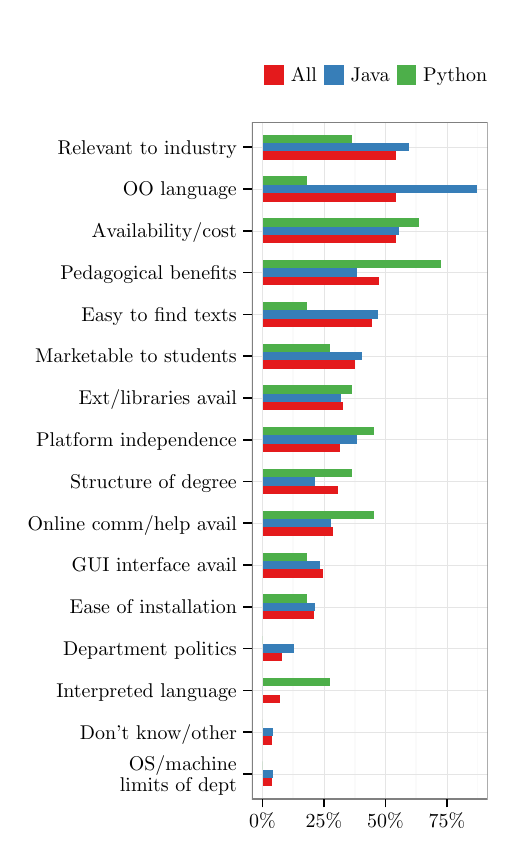
\begin{tikzpicture}[x=1pt,y=1pt]
\definecolor{fillColor}{RGB}{255,255,255}
\path[use as bounding box,fill=fillColor,fill opacity=0.00] (0,0) rectangle (166.22,289.08);
\begin{scope}
\path[clip] (  0.00,  0.00) rectangle (166.22,289.08);
\definecolor{drawColor}{RGB}{255,255,255}
\definecolor{fillColor}{RGB}{255,255,255}

\path[draw=drawColor,line width= 0.6pt,line join=round,line cap=round,fill=fillColor] (  0.00,  0.00) rectangle (166.22,289.08);
\end{scope}
\begin{scope}
\path[clip] ( 80.98, 10.36) rectangle (166.22,254.94);
\definecolor{fillColor}{RGB}{255,255,255}

\path[fill=fillColor] ( 80.98, 10.36) rectangle (166.22,254.94);
\definecolor{drawColor}{gray}{0.98}

\path[draw=drawColor,line width= 0.6pt,line join=round] ( 95.96, 10.36) --
	( 95.96,254.94);

\path[draw=drawColor,line width= 0.6pt,line join=round] (118.17, 10.36) --
	(118.17,254.94);

\path[draw=drawColor,line width= 0.6pt,line join=round] (140.38, 10.36) --
	(140.38,254.94);

\path[draw=drawColor,line width= 0.6pt,line join=round] (162.59, 10.36) --
	(162.59,254.94);
\definecolor{drawColor}{gray}{0.90}

\path[draw=drawColor,line width= 0.2pt,line join=round] ( 80.98, 19.42) --
	(166.22, 19.42);

\path[draw=drawColor,line width= 0.2pt,line join=round] ( 80.98, 34.51) --
	(166.22, 34.51);

\path[draw=drawColor,line width= 0.2pt,line join=round] ( 80.98, 49.61) --
	(166.22, 49.61);

\path[draw=drawColor,line width= 0.2pt,line join=round] ( 80.98, 64.71) --
	(166.22, 64.71);

\path[draw=drawColor,line width= 0.2pt,line join=round] ( 80.98, 79.81) --
	(166.22, 79.81);

\path[draw=drawColor,line width= 0.2pt,line join=round] ( 80.98, 94.90) --
	(166.22, 94.90);

\path[draw=drawColor,line width= 0.2pt,line join=round] ( 80.98,110.00) --
	(166.22,110.00);

\path[draw=drawColor,line width= 0.2pt,line join=round] ( 80.98,125.10) --
	(166.22,125.10);

\path[draw=drawColor,line width= 0.2pt,line join=round] ( 80.98,140.20) --
	(166.22,140.20);

\path[draw=drawColor,line width= 0.2pt,line join=round] ( 80.98,155.29) --
	(166.22,155.29);

\path[draw=drawColor,line width= 0.2pt,line join=round] ( 80.98,170.39) --
	(166.22,170.39);

\path[draw=drawColor,line width= 0.2pt,line join=round] ( 80.98,185.49) --
	(166.22,185.49);

\path[draw=drawColor,line width= 0.2pt,line join=round] ( 80.98,200.59) --
	(166.22,200.59);

\path[draw=drawColor,line width= 0.2pt,line join=round] ( 80.98,215.68) --
	(166.22,215.68);

\path[draw=drawColor,line width= 0.2pt,line join=round] ( 80.98,230.78) --
	(166.22,230.78);

\path[draw=drawColor,line width= 0.2pt,line join=round] ( 80.98,245.88) --
	(166.22,245.88);

\path[draw=drawColor,line width= 0.2pt,line join=round] ( 84.86, 10.36) --
	( 84.86,254.94);

\path[draw=drawColor,line width= 0.2pt,line join=round] (107.06, 10.36) --
	(107.06,254.94);

\path[draw=drawColor,line width= 0.2pt,line join=round] (129.27, 10.36) --
	(129.27,254.94);

\path[draw=drawColor,line width= 0.2pt,line join=round] (151.48, 10.36) --
	(151.48,254.94);
\definecolor{fillColor}{RGB}{228,26,28}

\path[fill=fillColor] ( 84.86, 14.89) rectangle ( 88.37, 17.91);
\definecolor{fillColor}{RGB}{55,126,184}

\path[fill=fillColor] ( 84.86, 17.91) rectangle ( 88.64, 20.93);
\definecolor{fillColor}{RGB}{77,175,74}

\path[fill=fillColor] ( 84.86, 20.93) rectangle ( 84.86, 23.95);
\definecolor{fillColor}{RGB}{228,26,28}

\path[fill=fillColor] ( 84.86, 29.99) rectangle ( 88.37, 33.00);
\definecolor{fillColor}{RGB}{55,126,184}

\path[fill=fillColor] ( 84.86, 33.00) rectangle ( 88.64, 36.02);
\definecolor{fillColor}{RGB}{77,175,74}

\path[fill=fillColor] ( 84.86, 36.02) rectangle ( 84.86, 39.04);
\definecolor{fillColor}{RGB}{228,26,28}

\path[fill=fillColor] ( 84.86, 45.08) rectangle ( 91.01, 48.10);
\definecolor{fillColor}{RGB}{55,126,184}

\path[fill=fillColor] ( 84.86, 48.10) rectangle ( 84.86, 51.12);
\definecolor{fillColor}{RGB}{77,175,74}

\path[fill=fillColor] ( 84.86, 51.12) rectangle (109.08, 54.14);
\definecolor{fillColor}{RGB}{228,26,28}

\path[fill=fillColor] ( 84.86, 60.18) rectangle ( 91.89, 63.20);
\definecolor{fillColor}{RGB}{55,126,184}

\path[fill=fillColor] ( 84.86, 63.20) rectangle ( 96.20, 66.22);
\definecolor{fillColor}{RGB}{77,175,74}

\path[fill=fillColor] ( 84.86, 66.22) rectangle ( 84.86, 69.24);
\definecolor{fillColor}{RGB}{228,26,28}

\path[fill=fillColor] ( 84.86, 75.28) rectangle (103.32, 78.30);
\definecolor{fillColor}{RGB}{55,126,184}

\path[fill=fillColor] ( 84.86, 78.30) rectangle (103.76, 81.32);
\definecolor{fillColor}{RGB}{77,175,74}

\path[fill=fillColor] ( 84.86, 81.32) rectangle (101.01, 84.34);
\definecolor{fillColor}{RGB}{228,26,28}

\path[fill=fillColor] ( 84.86, 90.38) rectangle (106.84, 93.39);
\definecolor{fillColor}{RGB}{55,126,184}

\path[fill=fillColor] ( 84.86, 93.39) rectangle (105.64, 96.41);
\definecolor{fillColor}{RGB}{77,175,74}

\path[fill=fillColor] ( 84.86, 96.41) rectangle (101.01, 99.43);
\definecolor{fillColor}{RGB}{228,26,28}

\path[fill=fillColor] ( 84.86,105.47) rectangle (110.36,108.49);
\definecolor{fillColor}{RGB}{55,126,184}

\path[fill=fillColor] ( 84.86,108.49) rectangle (109.43,111.51);
\definecolor{fillColor}{RGB}{77,175,74}

\path[fill=fillColor] ( 84.86,111.51) rectangle (125.23,114.53);
\definecolor{fillColor}{RGB}{228,26,28}

\path[fill=fillColor] ( 84.86,120.57) rectangle (112.12,123.59);
\definecolor{fillColor}{RGB}{55,126,184}

\path[fill=fillColor] ( 84.86,123.59) rectangle (103.76,126.61);
\definecolor{fillColor}{RGB}{77,175,74}

\path[fill=fillColor] ( 84.86,126.61) rectangle (117.16,129.63);
\definecolor{fillColor}{RGB}{228,26,28}

\path[fill=fillColor] ( 84.86,135.67) rectangle (113.00,138.69);
\definecolor{fillColor}{RGB}{55,126,184}

\path[fill=fillColor] ( 84.86,138.69) rectangle (118.88,141.71);
\definecolor{fillColor}{RGB}{77,175,74}

\path[fill=fillColor] ( 84.86,141.71) rectangle (125.23,144.73);
\definecolor{fillColor}{RGB}{228,26,28}

\path[fill=fillColor] ( 84.86,150.76) rectangle (113.88,153.78);
\definecolor{fillColor}{RGB}{55,126,184}

\path[fill=fillColor] ( 84.86,153.78) rectangle (113.20,156.80);
\definecolor{fillColor}{RGB}{77,175,74}

\path[fill=fillColor] ( 84.86,156.80) rectangle (117.16,159.82);
\definecolor{fillColor}{RGB}{228,26,28}

\path[fill=fillColor] ( 84.86,165.86) rectangle (118.28,168.88);
\definecolor{fillColor}{RGB}{55,126,184}

\path[fill=fillColor] ( 84.86,168.88) rectangle (120.77,171.90);
\definecolor{fillColor}{RGB}{77,175,74}

\path[fill=fillColor] ( 84.86,171.90) rectangle (109.08,174.92);
\definecolor{fillColor}{RGB}{228,26,28}

\path[fill=fillColor] ( 84.86,180.96) rectangle (124.43,183.98);
\definecolor{fillColor}{RGB}{55,126,184}

\path[fill=fillColor] ( 84.86,183.98) rectangle (126.44,187.00);
\definecolor{fillColor}{RGB}{77,175,74}

\path[fill=fillColor] ( 84.86,187.00) rectangle (101.01,190.02);
\definecolor{fillColor}{RGB}{228,26,28}

\path[fill=fillColor] ( 84.86,196.06) rectangle (127.07,199.08);
\definecolor{fillColor}{RGB}{55,126,184}

\path[fill=fillColor] ( 84.86,199.08) rectangle (118.88,202.10);
\definecolor{fillColor}{RGB}{77,175,74}

\path[fill=fillColor] ( 84.86,202.10) rectangle (149.47,205.12);
\definecolor{fillColor}{RGB}{228,26,28}

\path[fill=fillColor] ( 84.86,211.15) rectangle (133.24,214.17);
\definecolor{fillColor}{RGB}{55,126,184}

\path[fill=fillColor] ( 84.86,214.17) rectangle (134.00,217.19);
\definecolor{fillColor}{RGB}{77,175,74}

\path[fill=fillColor] ( 84.86,217.19) rectangle (141.39,220.21);
\definecolor{fillColor}{RGB}{228,26,28}

\path[fill=fillColor] ( 84.86,226.25) rectangle (133.24,229.27);
\definecolor{fillColor}{RGB}{55,126,184}

\path[fill=fillColor] ( 84.86,229.27) rectangle (162.35,232.29);
\definecolor{fillColor}{RGB}{77,175,74}

\path[fill=fillColor] ( 84.86,232.29) rectangle (101.01,235.31);
\definecolor{fillColor}{RGB}{228,26,28}

\path[fill=fillColor] ( 84.86,241.35) rectangle (133.24,244.37);
\definecolor{fillColor}{RGB}{55,126,184}

\path[fill=fillColor] ( 84.86,244.37) rectangle (137.77,247.39);
\definecolor{fillColor}{RGB}{77,175,74}

\path[fill=fillColor] ( 84.86,247.39) rectangle (117.16,250.41);
\definecolor{drawColor}{gray}{0.50}

\path[draw=drawColor,line width= 0.6pt,line join=round,line cap=round] ( 80.98, 10.36) rectangle (166.22,254.94);
\end{scope}
\begin{scope}
\path[clip] (  0.00,  0.00) rectangle (166.22,289.08);
\definecolor{drawColor}{RGB}{0,0,0}

\node[text=drawColor,anchor=base east,inner sep=0pt, outer sep=0pt, scale=  0.72] at ( 75.58, 20.83) {OS/machine};

\node[text=drawColor,anchor=base east,inner sep=0pt, outer sep=0pt, scale=  0.72] at ( 75.58, 13.05) {limits of dept};

\node[text=drawColor,anchor=base east,inner sep=0pt, outer sep=0pt, scale=  0.72] at ( 75.58, 32.04) {Don't know/other};

\node[text=drawColor,anchor=base east,inner sep=0pt, outer sep=0pt, scale=  0.72] at ( 75.58, 47.13) {Interpreted language};

\node[text=drawColor,anchor=base east,inner sep=0pt, outer sep=0pt, scale=  0.72] at ( 75.58, 62.23) {Department politics};

\node[text=drawColor,anchor=base east,inner sep=0pt, outer sep=0pt, scale=  0.72] at ( 75.58, 77.33) {Ease of installation};

\node[text=drawColor,anchor=base east,inner sep=0pt, outer sep=0pt, scale=  0.72] at ( 75.58, 92.42) {GUI interface avail};

\node[text=drawColor,anchor=base east,inner sep=0pt, outer sep=0pt, scale=  0.72] at ( 75.58,107.52) {Online comm/help avail};

\node[text=drawColor,anchor=base east,inner sep=0pt, outer sep=0pt, scale=  0.72] at ( 75.58,122.62) {Structure of degree};

\node[text=drawColor,anchor=base east,inner sep=0pt, outer sep=0pt, scale=  0.72] at ( 75.58,137.72) {Platform independence};

\node[text=drawColor,anchor=base east,inner sep=0pt, outer sep=0pt, scale=  0.72] at ( 75.58,152.81) {Ext/libraries avail};

\node[text=drawColor,anchor=base east,inner sep=0pt, outer sep=0pt, scale=  0.72] at ( 75.58,167.91) {Marketable to students};

\node[text=drawColor,anchor=base east,inner sep=0pt, outer sep=0pt, scale=  0.72] at ( 75.58,183.01) {Easy to find texts};

\node[text=drawColor,anchor=base east,inner sep=0pt, outer sep=0pt, scale=  0.72] at ( 75.58,198.11) {Pedagogical benefits};

\node[text=drawColor,anchor=base east,inner sep=0pt, outer sep=0pt, scale=  0.72] at ( 75.58,213.20) {Availability/cost};

\node[text=drawColor,anchor=base east,inner sep=0pt, outer sep=0pt, scale=  0.72] at ( 75.58,228.30) {OO language};

\node[text=drawColor,anchor=base east,inner sep=0pt, outer sep=0pt, scale=  0.72] at ( 75.58,243.40) {Relevant to industry};
\end{scope}
\begin{scope}
\path[clip] (  0.00,  0.00) rectangle (166.22,289.08);
\definecolor{drawColor}{RGB}{0,0,0}

\path[draw=drawColor,line width= 0.6pt,line join=round] ( 77.98, 19.42) --
	( 80.98, 19.42);

\path[draw=drawColor,line width= 0.6pt,line join=round] ( 77.98, 34.51) --
	( 80.98, 34.51);

\path[draw=drawColor,line width= 0.6pt,line join=round] ( 77.98, 49.61) --
	( 80.98, 49.61);

\path[draw=drawColor,line width= 0.6pt,line join=round] ( 77.98, 64.71) --
	( 80.98, 64.71);

\path[draw=drawColor,line width= 0.6pt,line join=round] ( 77.98, 79.81) --
	( 80.98, 79.81);

\path[draw=drawColor,line width= 0.6pt,line join=round] ( 77.98, 94.90) --
	( 80.98, 94.90);

\path[draw=drawColor,line width= 0.6pt,line join=round] ( 77.98,110.00) --
	( 80.98,110.00);

\path[draw=drawColor,line width= 0.6pt,line join=round] ( 77.98,125.10) --
	( 80.98,125.10);

\path[draw=drawColor,line width= 0.6pt,line join=round] ( 77.98,140.20) --
	( 80.98,140.20);

\path[draw=drawColor,line width= 0.6pt,line join=round] ( 77.98,155.29) --
	( 80.98,155.29);

\path[draw=drawColor,line width= 0.6pt,line join=round] ( 77.98,170.39) --
	( 80.98,170.39);

\path[draw=drawColor,line width= 0.6pt,line join=round] ( 77.98,185.49) --
	( 80.98,185.49);

\path[draw=drawColor,line width= 0.6pt,line join=round] ( 77.98,200.59) --
	( 80.98,200.59);

\path[draw=drawColor,line width= 0.6pt,line join=round] ( 77.98,215.68) --
	( 80.98,215.68);

\path[draw=drawColor,line width= 0.6pt,line join=round] ( 77.98,230.78) --
	( 80.98,230.78);

\path[draw=drawColor,line width= 0.6pt,line join=round] ( 77.98,245.88) --
	( 80.98,245.88);
\end{scope}
\begin{scope}
\path[clip] (  0.00,  0.00) rectangle (166.22,289.08);
\definecolor{drawColor}{RGB}{0,0,0}

\path[draw=drawColor,line width= 0.6pt,line join=round] ( 84.86,  7.36) --
	( 84.86, 10.36);

\path[draw=drawColor,line width= 0.6pt,line join=round] (107.06,  7.36) --
	(107.06, 10.36);

\path[draw=drawColor,line width= 0.6pt,line join=round] (129.27,  7.36) --
	(129.27, 10.36);

\path[draw=drawColor,line width= 0.6pt,line join=round] (151.48,  7.36) --
	(151.48, 10.36);
\end{scope}
\begin{scope}
\path[clip] (  0.00,  0.00) rectangle (166.22,289.08);
\definecolor{drawColor}{RGB}{0,0,0}

\node[text=drawColor,anchor=base,inner sep=0pt, outer sep=0pt, scale=  0.72] at ( 84.86, -0.00) {0\%};

\node[text=drawColor,anchor=base,inner sep=0pt, outer sep=0pt, scale=  0.72] at (107.06, -0.00) {25\%};

\node[text=drawColor,anchor=base,inner sep=0pt, outer sep=0pt, scale=  0.72] at (129.27, -0.00) {50\%};

\node[text=drawColor,anchor=base,inner sep=0pt, outer sep=0pt, scale=  0.72] at (151.48, -0.00) {75\%};
\end{scope}
\begin{scope}
\path[clip] (  0.00,  0.00) rectangle (166.22,289.08);
\definecolor{fillColor}{RGB}{255,255,255}

\path[fill=fillColor] ( 76.91,263.47) rectangle (170.29,280.54);
\end{scope}
\begin{scope}
\path[clip] (  0.00,  0.00) rectangle (166.22,289.08);
\definecolor{fillColor}{RGB}{228,26,28}

\path[fill=fillColor] ( 85.50,268.45) rectangle ( 92.62,275.56);
\end{scope}
\begin{scope}
\path[clip] (  0.00,  0.00) rectangle (166.22,289.08);
\definecolor{fillColor}{RGB}{55,126,184}

\path[fill=fillColor] (107.05,268.45) rectangle (114.16,275.56);
\end{scope}
\begin{scope}
\path[clip] (  0.00,  0.00) rectangle (166.22,289.08);
\definecolor{fillColor}{RGB}{77,175,74}

\path[fill=fillColor] (133.30,268.45) rectangle (140.41,275.56);
\end{scope}
\begin{scope}
\path[clip] (  0.00,  0.00) rectangle (166.22,289.08);
\definecolor{drawColor}{RGB}{0,0,0}

\node[text=drawColor,anchor=base west,inner sep=0pt, outer sep=0pt, scale=  0.72] at ( 95.14,269.53) {All};
\end{scope}
\begin{scope}
\path[clip] (  0.00,  0.00) rectangle (166.22,289.08);
\definecolor{drawColor}{RGB}{0,0,0}

\node[text=drawColor,anchor=base west,inner sep=0pt, outer sep=0pt, scale=  0.72] at (116.68,269.53) {Java};
\end{scope}
\begin{scope}
\path[clip] (  0.00,  0.00) rectangle (166.22,289.08);
\definecolor{drawColor}{RGB}{0,0,0}

\node[text=drawColor,anchor=base west,inner sep=0pt, outer sep=0pt, scale=  0.72] at (142.93,269.53) {Python};
\end{scope}
\end{tikzpicture}
